\documentclass{article}
Gronenschild2012,Glatard2015,Scaria2017,Glasser2013,Chirigati2016
\usepackage{pdfcomment}
\usepackage[margin=1in]{geometry}
\usepackage{xcolor}
\usepackage{graphicx}

\newcommand{\note}[2]{\pdfmargincomment[color=yellow,author=#1,open=true]{#2}}
\newcommand{\todo}[2]{\pdfmargincomment[color=red,author=#1,open=true]{#2}}

\title{Numerical error propagation in the HCP structural pre-processing pipelines}

\author{M. Ali Salari, Lalet Scaria, Gregory Kiar, Tristan Glatard}

\begin{document}

\maketitle

\abstract{}

\section{Introduction}

Operating systems are known to have an effect on the results produced by neuroimaging pipelines~\cite{Gronenschild2012, Glatard2015}, 
presumably due to the creation, propagation and amplification of small numerical errors across the pipelines. 
Such errors highlight numerical instability which is also likely to appear as a result of other types of small 
perturbations such as acquisition and parametric noise. In a previous study~\cite{Scaria2017}, 
we showed that pre-processing pipelines of the Human Connectome Project~\cite{Glasser2013} were sensitive to operating system variation (see Figure \ref{fig:1}). 
However, the precise causes of such instabilities and the path along which they propagate in the pipelines are unclear. 
We present a technique to identify the processes in a pipeline that create numerical errors along the execution, 
and we apply this technique to the HCP structural pre-processing pipelines. 

\begin{figure}
  \includegraphics[width=\linewidth]{brain_classificatio}
  \caption{Tissue classification produced by the HCP pre-processing pipelines on subject 105216 (CentOS 6 vs CentOS 7).}
  \label{fig:1}
\end{figure}


 \emph{et al.}

\todo{Link this to Lindsay's HBM 2017 poster and to Redolfi et al.}

\section{Methods}

We randomly selected 6 subjects from the HCP data release S500 and processed them with 
the HCP structural pre-processing pipelines v3.19.0 (PreFreeSurfer and FreeSurfer)~\cite{Glasser2013} 
in CentOS 6.8 and CentOS 7.2 using Docker containers. We collected the provenance trace 
(tree of executed processes and files accessed in read or write mode) for one subject 
using system-call interception as provided by the reprozip tool~\cite{5}. We computed a file difference matrix 
between files produced in each operating system based on file checksums as in~\cite{Scaria2017}.
From the reprozip trace and file error matrix, we classified processes depending whether they created errors, 
removed errors, or did not have any impact. To control the propagation of errors in the pipeline and allow 
for the classification of all processes, process classification was done in an iterative manner in which we 
artificially corrected errors by replacing the original process by a file copy from the results obtained 
in the other operating system. In this way, we were able to pinpoint the origin of the errors measured in the pipeline. 

\section{Results}

Among the 117 data files produced by PreFreeSurfer, 23 did not have any error for any subject, 92 had errors 
for all subjects and 2 had errors for 1 subject only. 
Figure \ref{fig:2} shows the annotated provenance graph of the PreFreeSurfer pipeline executed on CentOS6 and CentOS7. 
Processes that created errors are shown in red, processes that removed errors are in blue, and other processes are in green. 
Squares denote processes for which the classification is uncertain. Black edges link sub-processes to their parents while 
dashed edges denote file dependencies between processes (green edges: files with no errors; red edges: files with errors; yellow edges: temporary files).  
The processes that introduce errors in PreFreeSurfer are: linear registration with “\emph{FLIRT}” 
(8 occurrences, in ACPC Alignment, BrainExtraction, DistortionCorrection, AtlasRegistration), 
non-linear registration with “\emph{FNIRT}” (3 occurrences, in BrainExtraction and AltasRegistration), 
image warping with “\emph{new_invwarp}” (3 occurrences, in BrainExtraction and AtlasRegistration). 
In addition, errors were observed in image mean and standard-deviation computations with “\emph{fslstats}” (3 occurrences in BiasFieldCorrection), 
and in masked image extrapolation with “\emph{fslmaths}” (1 occurrence, in BiasFieldCorrection). 
Besides, transformation format conversion with “\emph{convertwarp}” (2 occurrences, in DistortionCorrection) was able to remove errors. 

\begin{figure}
  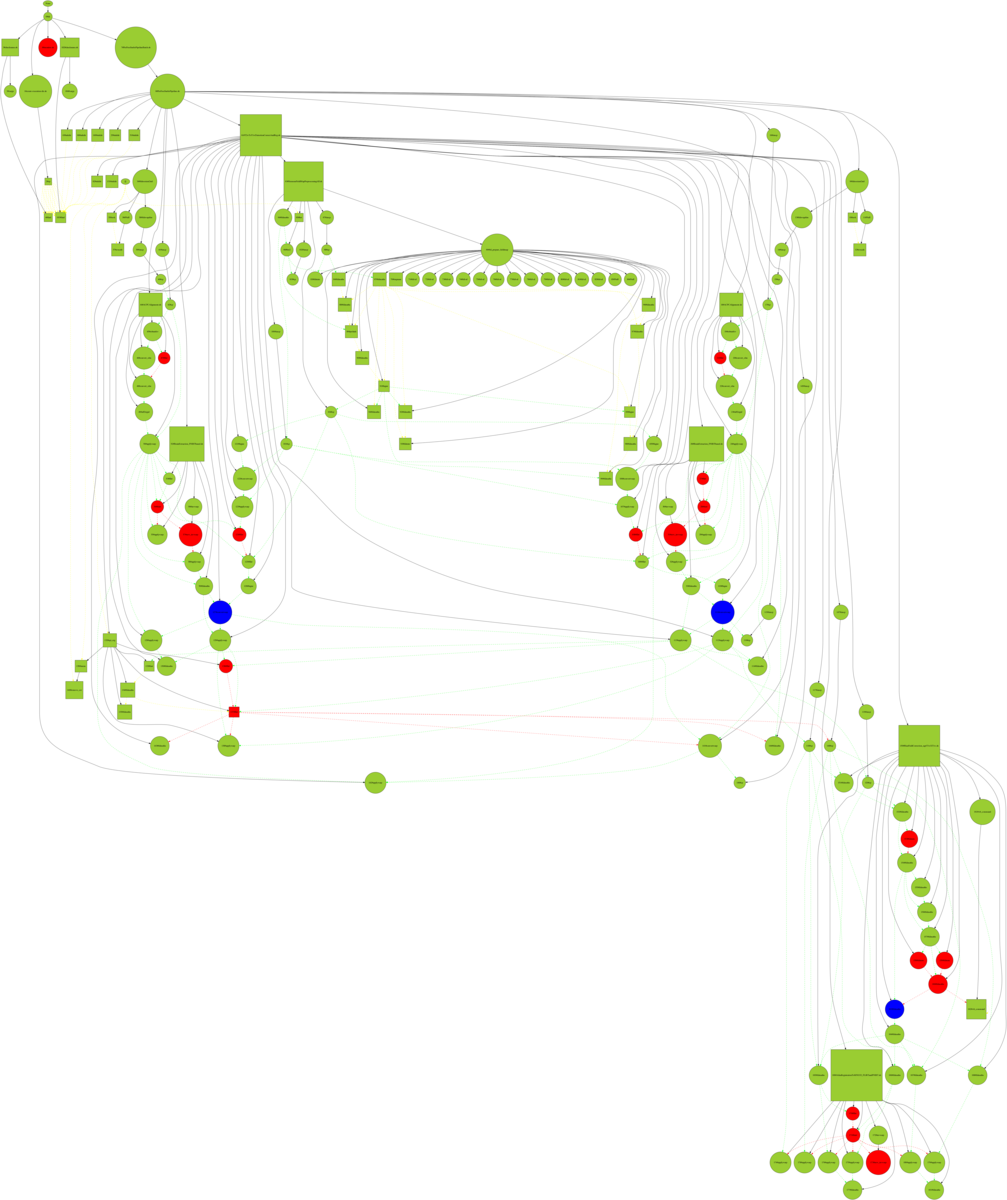
\includegraphics[width=\linewidth]{graph}
  \caption{An annotated provenance graph from the PreFreesurfer pipeline. Processes that created errors are in red. 
Full-resolution image available at \url{https://drive.google.com/open?id=174yyn8SuVOUcK5aRVw0bagjDanLD0FLt}.}
  \label{fig:2}
\end{figure}

\section{Conclusion}

The numerical instability in the PreFreesurfer HCP pipeline arises mainly from linear and non-linear registration processes 
implemented in FSL FLIRT and FNIRT. These processes need to be reviewed to understand and correct the cause of instabilities. 
In this correction process, accuracy has to be considered in addition to stability. Our technique is able to 
characterize the stability of a pipeline’s components automatically, but it also suffers from limitations as it cannot deal with: 
(1) results that are not written to disk (values processed in memory); (2) temporary files (3) files that are written by more than one process.


\section{Acknowledgments}



\bibliographystyle{plain}
\bibliography{biblio_OHBM}

\end{document}
